\chapter{Motion in a Plane: Projectiles and Circles}
\label{ch:plane}
\begin{chapterintro}
\textbf{You will learn to:} analyse projectile motion with constant acceleration;
compute range, maximum height, and time of flight; describe circular motion with
angular velocity and centripetal acceleration; and handle non-uniform circular
motion.
\end{chapterintro}

\section{Projectile motion}

Take the $y$-axis vertical and neglect air resistance. The only acceleration is
\[
a_x=0,\qquad a_y=-g.
\]
With initial speed $v_0$ at angle $\alpha$ above the horizontal:
\[
x(t)=(v_0\cos\alpha)t,\qquad
y(t)=(v_0\sin\alpha)t-\frac12gt^2.
\]
Eliminating $t$,
\[
y(x)=x\tan\alpha-\frac{gx^2}{2v_0^2\cos^2\alpha}.
\]
The trajectory is a parabola.

For a projectile launched and landing at the same height:
\[
T=\frac{2v_0\sin\alpha}{g},
\qquad
R=\frac{v_0^2\sin2\alpha}{g},
\qquad
H=\frac{v_0^2\sin^2\alpha}{2g}.
\]
The range is maximum at $\alpha=45^\circ$, where $R_{\max}=v_0^2/g$.

\begin{figure}[htbp]
\centering
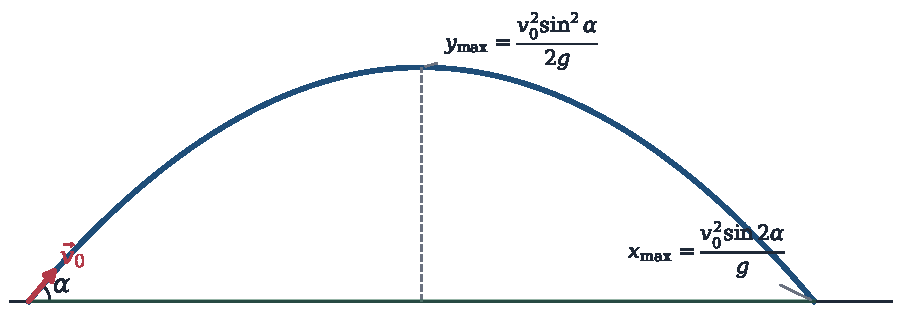
\includegraphics[width=0.9\textwidth]{figures/06_projectile.pdf}
\caption{Projectile motion: the velocity is tangent to the parabola, while the
acceleration is always vertically downward.}
\label{fig:projectile}
\end{figure}

\begin{warning}[Two frequent mistakes]
The horizontal velocity never changes (no air resistance), and the vertical
acceleration is $g$ even at the highest point. ``$a=0$ at the top'' is false:
only $v_y=0$ there.
\end{warning}

\section{Circular motion}

For a particle moving on a circle of radius $R$, let $\theta(t)$ be its angular
position. Define
\[
\omega=\dot\theta\quad(\mathrm{rad\,s^{-1}}),\qquad
\alpha=\dot\omega=\ddot\theta\quad(\mathrm{rad\,s^{-2}}).
\]
Then
\[
v=R\omega,\qquad
a_t=R\alpha,\qquad
a_n=\frac{v^2}{R}=R\omega^2.
\]
The tangential acceleration $a_t$ changes the speed; the normal (centripetal)
acceleration $a_n$ changes the direction and always points toward the centre.
The total acceleration has magnitude
\[
a=\sqrt{a_t^2+a_n^2}.
\]
The period of uniform circular motion is $T=2\pi/\omega$.

\begin{figure}[htbp]
\centering
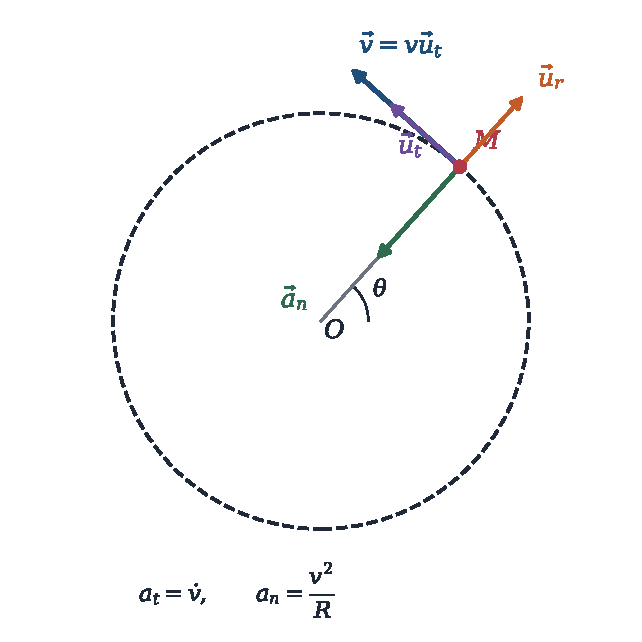
\includegraphics[width=0.68\textwidth]{figures/07_circular_motion.pdf}
\caption{Circular motion. The velocity is tangential; the centripetal
acceleration points toward the centre.}
\label{fig:circular}
\end{figure}

\begin{keyidea}[Intrinsic decomposition]
For any curved path, with $\utt$ the unit tangent and $\un$ the unit normal
pointing toward the centre of curvature,
\[
\vec a=\frac{\dd v}{\dd t}\utt+\frac{v^2}{R}\un.
\]
For a circle, $R$ is constant; for a general curve, $R$ is the local radius of
curvature.
\end{keyidea}

% ===========================================================================
\section{Worked examples}

\begin{worked}[Full projectile analysis]
A projectile is launched from the ground with $v_0=25.0\ \mathrm{m\,s^{-1}}$ at
$\alpha=40.0^\circ$. Find the time of flight, the range, the maximum height, and
the velocity at $t=1.50\ \mathrm{s}$.
\end{worked}

\begin{solution}{5.1}
\[
v_{0x}=25.0\cos40.0^\circ=19.2\ \mathrm{m\,s^{-1}},\qquad
v_{0y}=25.0\sin40.0^\circ=16.1\ \mathrm{m\,s^{-1}}.
\]
Time of flight:
\[
T=\frac{2v_{0y}}{g}=\frac{32.1}{9.81}=3.28\ \mathrm{s}.
\]
Range:
\[
R=v_{0x}T=(19.2)(3.28)=62.9\ \mathrm{m},
\]
or directly $R=v_0^2\sin80^\circ/g=62.7\ \mathrm{m}$.

Maximum height:
\[
H=\frac{v_{0y}^2}{2g}=\frac{258}{19.62}=13.2\ \mathrm{m}.
\]
At $t=1.50\ \mathrm{s}$:
\[
v_x=19.2\ \mathrm{m\,s^{-1}},\qquad
v_y=16.1-9.81(1.50)=1.36\ \mathrm{m\,s^{-1}},
\]
\[
v=\sqrt{19.2^2+1.36^2}=19.2\ \mathrm{m\,s^{-1}}.
\]
The projectile is still rising slightly.
\end{solution}

\begin{worked}[Non-uniform circular motion]
A particle moves on a circle of radius $R=0.500\ \mathrm{m}$ with angular
position $\theta(t)=2t^2$ (rad). At $t=1.00\ \mathrm{s}$, find the angular
velocity, angular acceleration, speed, tangential and normal accelerations, and
the total acceleration.
\end{worked}

\begin{solution}{5.2}
\[
\omega=\dot\theta=4t,\qquad \alpha=\dot\omega=4.
\]
At $t=1$: $\omega=4.00\ \mathrm{rad\,s^{-1}}$, $\alpha=4.00\ \mathrm{rad\,s^{-2}}$.

\[
v=R\omega=0.500(4.00)=2.00\ \mathrm{m\,s^{-1}},
\]
\[
a_t=R\alpha=0.500(4.00)=2.00\ \mathrm{m\,s^{-2}},
\]
\[
a_n=R\omega^2=0.500(16.0)=8.00\ \mathrm{m\,s^{-2}}.
\]
\[
a=\sqrt{2.00^2+8.00^2}=\sqrt{68.0}=8.25\ \mathrm{m\,s^{-2}}.
\]
\end{solution}

% ===========================================================================
\section{Exercises and Step-by-Step Solutions}

\begin{exercise}{\warm\ Basic projectile}
A ball is launched from the ground with $v_0=20.0\ \mathrm{m\,s^{-1}}$ at
$30.0^\circ$ above the horizontal. Find the time of flight, the range, and the
maximum height.
\end{exercise}

\begin{tabletworkspace}[6.5cm]
\end{tabletworkspace}

\begin{solution}{5.1}
\[
v_{0x}=20.0\cos30.0^\circ=17.3\ \mathrm{m\,s^{-1}},\qquad
v_{0y}=20.0\sin30.0^\circ=10.0\ \mathrm{m\,s^{-1}}.
\]
\[
T=\frac{2v_{0y}}{g}=\frac{20.0}{9.81}=2.04\ \mathrm{s}.
\]
\[
R=v_{0x}T=(17.3)(2.04)=35.3\ \mathrm{m}.
\]
\[
H=\frac{v_{0y}^2}{2g}=\frac{100}{19.62}=5.10\ \mathrm{m}.
\]
\end{solution}

\begin{exercise}{\warm\ Horizontal launch}
A ball is thrown horizontally from a cliff of height $20.0\ \mathrm{m}$ with
speed $15.0\ \mathrm{m\,s^{-1}}$. Find the time to reach the ground, the
horizontal distance travelled, and the impact speed.
\end{exercise}

\begin{tabletworkspace}[6.5cm]
\end{tabletworkspace}

\begin{solution}{5.2}
Vertical motion (downward positive):
\[
h=\frac12gt^2
\implies
t=\sqrt{\frac{2(20.0)}{9.81}}=2.02\ \mathrm{s}.
\]
Horizontal distance:
\[
x=v_0t=15.0(2.02)=30.3\ \mathrm{m}.
\]
Impact velocity:
\[
v_x=15.0,\qquad v_y=gt=19.8\ \mathrm{m\,s^{-1}},
\]
\[
v=\sqrt{15.0^2+19.8^2}=24.9\ \mathrm{m\,s^{-1}}.
\]
\end{solution}

\begin{exercise}{\warm\ Uniform circular motion}
A point moves on a circle of radius $2.00\ \mathrm{m}$ with period
$0.500\ \mathrm{s}$. Find its angular velocity, speed, and centripetal
acceleration.
\end{exercise}

\begin{tabletworkspace}[6.5cm]
\end{tabletworkspace}

\begin{solution}{5.3}
\[
\omega=\frac{2\pi}{T}=\frac{2\pi}{0.500}=12.6\ \mathrm{rad\,s^{-1}}.
\]
\[
v=R\omega=2.00(12.6)=25.1\ \mathrm{m\,s^{-1}}.
\]
\[
a_n=\frac{v^2}{R}=\frac{631}{2.00}=316\ \mathrm{m\,s^{-2}}.
\]
\end{solution}

\begin{exercise}{\core\ Range and maximum height}
A projectile launched at $45.0^\circ$ has a range of $100\ \mathrm{m}$. Find its
initial speed, maximum height, and time of flight.
\end{exercise}

\begin{tabletworkspace}[6.5cm]
\end{tabletworkspace}

\begin{solution}{5.4}
For $\alpha=45^\circ$, $\sin2\alpha=1$, so
\[
R=\frac{v_0^2}{g}
\implies
v_0=\sqrt{gR}=\sqrt{9.81(100)}=31.3\ \mathrm{m\,s^{-1}}.
\]
\[
H=\frac{v_0^2\sin^245^\circ}{2g}
=\frac{gR(1/2)}{2g}=\frac R4=25.0\ \mathrm{m}.
\]
\[
T=\frac{2v_0\sin45^\circ}{g}
=\frac{2(31.3)(0.707)}{9.81}=4.51\ \mathrm{s}.
\]
\end{solution}

\begin{exercise}{\core\ Clearing a wall}
A projectile is launched with $v_0=30.0\ \mathrm{m\,s^{-1}}$ at $50.0^\circ$.
A wall stands $60.0\ \mathrm{m}$ away. Does the projectile clear a wall of height
$10.0\ \mathrm{m}$? Find its height and velocity when it reaches the wall.
\end{exercise}

\begin{tabletworkspace}[6.5cm]
\end{tabletworkspace}

\begin{solution}{5.5}
\[
v_x=30.0\cos50.0^\circ=19.3\ \mathrm{m\,s^{-1}},\qquad
v_{0y}=30.0\sin50.0^\circ=23.0\ \mathrm{m\,s^{-1}}.
\]
Time to reach the wall:
\[
t=\frac{x}{v_x}=\frac{60.0}{19.3}=3.11\ \mathrm{s}.
\]
Height at that time:
\[
y=23.0(3.11)-\frac12(9.81)(3.11)^2
=71.5-47.4=24.1\ \mathrm{m}.
\]
This is well above $10.0\ \mathrm{m}$, so the projectile clears the wall.

Velocity at the wall:
\[
v_x=19.3,\qquad v_y=23.0-9.81(3.11)=-7.51\ \mathrm{m\,s^{-1}},
\]
\[
v=\sqrt{19.3^2+7.51^2}=20.7\ \mathrm{m\,s^{-1}},
\]
directed $21.3^\circ$ below the horizontal (the projectile is descending).
\end{solution}

\begin{exercise}{\core\ Speed at the top}
A projectile is launched at angle $\theta$ above the horizontal. At the highest
point its speed is exactly half its initial speed. Find $\theta$.
\end{exercise}

\begin{tabletworkspace}[6.5cm]
\end{tabletworkspace}

\begin{solution}{5.6}
At the highest point $v_y=0$, so the speed is $v_x=v_0\cos\theta$. The condition
$v=v_0/2$ gives
\[
v_0\cos\theta=\frac{v_0}{2}
\implies
\cos\theta=\frac12
\implies
\theta=60.0^\circ.
\]
\end{solution}

\begin{exercise}{\core\ Two angles, one range}
A projectile has initial speed $30.0\ \mathrm{m\,s^{-1}}$ and must reach a range
of $80.0\ \mathrm{m}$. Find the two possible launch angles and the corresponding
times of flight.
\end{exercise}

\begin{tabletworkspace}[6.5cm]
\end{tabletworkspace}

\begin{solution}{5.7}
\[
R=\frac{v_0^2\sin2\theta}{g}
\implies
\sin2\theta=\frac{gR}{v_0^2}
=\frac{9.81(80.0)}{(30.0)^2}=0.872.
\]
Thus
\[
2\theta=60.7^\circ\ \text{or}\ 119.3^\circ,
\]
so
\[
\theta_1=30.4^\circ,\qquad \theta_2=59.6^\circ.
\]
The times of flight are
\[
T_1=\frac{2(30.0)\sin30.4^\circ}{9.81}=3.10\ \mathrm{s},
\]
\[
T_2=\frac{2(30.0)\sin59.6^\circ}{9.81}=5.28\ \mathrm{s}.
\]
The lower angle gives the shorter flight and the smaller maximum height.
\end{solution}

\begin{exercise}{\core\ Angular kinematics}
A particle moves on a circle of radius $R=0.500\ \mathrm{m}$ with angular
position $\theta(t)=2t^2$ rad. At $t=1.00\ \mathrm{s}$, find $\omega$, $\alpha$,
$v$, $a_t$, $a_n$, and the total acceleration.
\end{exercise}

\begin{tabletworkspace}[6.5cm]
\end{tabletworkspace}

\begin{solution}{5.8}
\[
\omega=\dot\theta=4t,\qquad \alpha=\dot\omega=4.
\]
At $t=1.00\ \mathrm{s}$:
\[
\omega=4.00\ \mathrm{rad\,s^{-1}},\qquad
\alpha=4.00\ \mathrm{rad\,s^{-2}}.
\]
\[
v=R\omega=0.500(4.00)=2.00\ \mathrm{m\,s^{-1}},
\]
\[
a_t=R\alpha=0.500(4.00)=2.00\ \mathrm{m\,s^{-2}},
\]
\[
a_n=R\omega^2=0.500(16.0)=8.00\ \mathrm{m\,s^{-2}}.
\]
\[
a=\sqrt{a_t^2+a_n^2}=\sqrt{4.00+64.0}=8.25\ \mathrm{m\,s^{-2}}.
\]
\end{solution}

\begin{exercise}{\mastery\ Deriving the range formula}
Starting from $x=v_0\cos\alpha\,t$ and
$y=v_0\sin\alpha\,t-\frac12gt^2$, derive
\[
y=x\tan\alpha-\frac{gx^2}{2v_0^2\cos^2\alpha},
\]
then show that for equal launch and landing heights the range is
$R=v_0^2\sin2\alpha/g$. Deduce that the maximum range occurs at $45^\circ$ and
that complementary angles give the same range.
\end{exercise}

\begin{tabletworkspace}[6.5cm]
\end{tabletworkspace}

\begin{solution}{5.9}
From $x=v_0\cos\alpha\,t$,
\[
t=\frac{x}{v_0\cos\alpha}.
\]
Substituting into $y$:
\[
y=v_0\sin\alpha\frac{x}{v_0\cos\alpha}
-\frac12g\frac{x^2}{v_0^2\cos^2\alpha}
=x\tan\alpha-\frac{gx^2}{2v_0^2\cos^2\alpha}.
\]
At landing, $y=0$ and $x=R$:
\[
R\tan\alpha=\frac{gR^2}{2v_0^2\cos^2\alpha}.
\]
For $R\ne0$,
\[
R=\frac{2v_0^2\sin\alpha\cos\alpha}{g}
=\frac{v_0^2\sin2\alpha}{g}.
\]
This is maximum when $\sin2\alpha=1$, i.e.\ $2\alpha=90^\circ$ and
$\alpha=45^\circ$, giving $R_{\max}=v_0^2/g$. Since
$\sin(180^\circ-2\alpha)=\sin2\alpha$, the angles $\alpha$ and
$90^\circ-\alpha$ give the same range.
\end{solution}

\begin{exercise}{\mastery\ Hitting a target}
A projectile is launched from the origin with speed
$v_0=25.0\ \mathrm{m\,s^{-1}}$ and must pass through the point
$(x,y)=(30.0,10.0)\ \mathrm{m}$. Using $u=\tan\alpha$, show that
\[
\frac{gx^2}{2v_0^2}u^2-xu+\left(y+\frac{gx^2}{2v_0^2}\right)=0,
\]
and find the two possible launch angles.
\end{exercise}

\begin{tabletworkspace}[6.5cm]
\end{tabletworkspace}

\begin{solution}{5.10}
With $u=\tan\alpha$ and
$\cos^2\alpha=1/(1+u^2)$,
\[
y=xu-\frac{gx^2}{2v_0^2}(1+u^2).
\]
Rearranging,
\[
\frac{gx^2}{2v_0^2}u^2-xu+\left(y+\frac{gx^2}{2v_0^2}\right)=0.
\]
For $x=30.0\ \mathrm{m}$, $y=10.0\ \mathrm{m}$, $v_0=25.0\ \mathrm{m\,s^{-1}}$:
\[
A=\frac{9.81(30.0)^2}{2(25.0)^2}=7.063,
\]
so
\[
7.063u^2-30.0u+17.063=0.
\]
\[
u=\frac{30.0\pm\sqrt{900-4(7.063)(17.063)}}{2(7.063)}
=\frac{30.0\pm20.44}{14.126}.
\]
Thus
\[
u_1=3.57\implies\alpha_1=74.4^\circ,\qquad
u_2=0.677\implies\alpha_2=34.1^\circ.
\]
Both trajectories pass through the target; the low-angle shot arrives sooner.
\end{solution}

